\documentclass[xcolor=table,dvipsnames,table]{beamer}
\mode<presentation>
\usetheme{boxes}
\setbeamertemplate{navigation symbols}{}
% http://www.latex-community.org/forum/viewtopic.php?f=4&t=6694
\setbeamertemplate{navigation symbols}{\raisebox{5pt}{\makebox[\paperwidth]{\hfill\makebox[10pt]{\scriptsize\insertframenumber\vspace{1ex}}}}}
%\setbeamertemplate{footline}[frame number]
\setbeamertemplate{blocks}[shadow=false]
%\setbeamercolor*{block title}{fg=structure,bg=RoyalBlue!10}
\setbeamercolor*{block title example}{fg=structure,bg=RoyalBlue!10}
%\setbeamercolor*{block title example}{fg=BrickRed,bg=Goldenrod!10}
\setbeamercolor*{block title alerted}{fg=white,bg=black}
\addtobeamertemplate{block begin}{\pgfsetfillopacity{0.8}}{\pgfsetfillopacity{1}}
%\rowcolors{0}{RoyalBlue!20}{RoyalBlue!5}

%\DeclareGraphicsRule{*}{mps}{*}{}

\usepackage{latexsym}
\usepackage{hyperref}
\usepackage{tikz}
\usetikzlibrary{calc,shapes,arrows,shadows,shapes.callouts,shapes.arrows,chains,positioning,trees}
\usepackage{solution}
\usepackage{calc}
\usepackage{pifont}
\usepackage{algorithmic}

\newcommand{\cmark}{\ding{51}}
\newcommand{\xmark}{\ding{55}}

\newcounter{mycallout}

\newcommand{\callouts}[3]{%
  \stepcounter{mycallout}
  \tikz[remember picture,baseline]{\node[anchor=base,inner sep=0,outer sep=0]%
    (\themycallout) {\colorbox{#1!20}{#3}};\pause\node[overlay,rectangle callout,%
    callout relative pointer={(0cm,0.5cm)},fill=#1!20] at ($(\themycallout.south)+(-0cm,-0.7cm)$){#2};}%
    }%

\raggedright

\newcount\lecturecount
\lecturecount=0
\AtBeginLecture{%
    \advance\lecturecount by 1
    \date{}
    \begin{frame}
    \begin{center}
    \titlepage
    \ifnum\lecturecount=1
    Part \the\lecturecount: \insertlecture
    \else
    Part \the\lecturecount: \insertlecture
    \fi
    \end{center}
    \end{frame}
}

\addtobeamertemplate{block begin}{\setlength\abovedisplayskip{0pt}}

%\newcommand{\example}[1]{{\color{BrickRed!50}{#1}}}
\newcommand{\maths}[1]{{\color{RoyalBlue!50}{#1}}}
\newcommand{\reference}[1]{{\color{RoyalBlue!30}\tiny [from #1]}}
\newcommand{\koehnref}{\reference{\href{http://www.statmt.org/book}{P.Koehn SMT book slides}}}


\begin{document}

\title{\color{RoyalBlue!20}Natural Language Processing}

\author{Anoop Sarkar \\ {\tt anoopsarkar.github.io/nlp-class}}
\institute{Simon Fraser University}
%\date{}
     
{
\setbeamertemplate{navigation symbols}{}
\addtocounter{framenumber}{-1}
\begin{frame}
\begin{center}
\vspace{8mm}
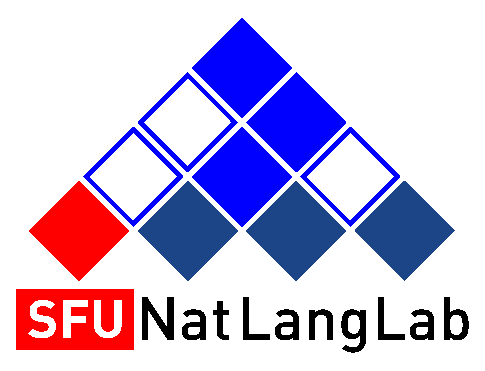
\includegraphics[scale=0.35]{figures/natlang-cky-logo}
\end{center}
\titlepage
\end{frame}
}



\lecture{Multi-layer perceptrons}
%\frame{\tableofcontents[currentsection]}

\begin{frame}{Log linear model}
\begin{itemize}[<+->]
\item Let there be $m$ features, $f_k(\textbf{x}, y)$ for $k = 1, \ldots, m$
\item Define a parameter vector $\textbf{v} \in \mathbb{R}^m$
\item A log-linear model for classification into labels $y \in {\cal Y}$: 
\[ \Pr(y \mid \textbf{x}; \textbf{v}) = \frac{exp\left(\textbf{v} \cdot \textbf{f}(\textbf{x}, y))\right)}{\sum_{y' \in {\cal Y}} exp\left(\textbf{v} \cdot \textbf{f}(\textbf{x}, y'))\right)} \]
\end{itemize}
\pause
\begin{block}{Advantages}
The feature representation $\textbf{f}(\textbf{x}, y)$ can represent any aspect of the input that is useful for classification.
\end{block}
\pause
\begin{block}{Disadvantages}
The feature representation $\textbf{f}(\textbf{x}, y)$ has to be designed by hand which is time-consuming and error-prone.
\end{block}
\end{frame}

\begin{frame}{Neural Networks}
\begin{block}{Advantages}
\begin{itemize}[<+->]
\item Neural networks replace hand-engineered features with \textbf{representation learning}
\item Empirical results across many different domains show that learned representations give significant improvements in accuracy
\item Neural networks allow end to end training for complex NLP tasks and do not have the limitations of multiple chained pipeline models 
\end{itemize}
\end{block}
\pause
\begin{block}{Disadvantages}
For many tasks linear models are much faster to train compared to neural network models
\end{block}
\end{frame}

\begin{frame}{Alternative Form of Log linear model}
\begin{block}{Log-linear model:}
\[ \Pr(y \mid \textbf{x}; \textbf{v}) = \frac{exp\left(\textbf{v} \cdot \textbf{f}(\textbf{x}, y))\right)}{\sum_{y' \in {\cal Y}} exp\left(\textbf{v} \cdot \textbf{f}(\textbf{x}, y'))\right)} \]
\end{block}

\begin{block}{Alternative form using functions:}
\[ \Pr(y \mid x; v) = \frac{exp\left(v(y) \cdot f(x) + \gamma_y \right)}{\sum_{y' \in {\cal Y}} exp\left(v(y') \cdot f(x) + \gamma_y')\right)} \]
\end{block}

\begin{itemize}[<+->]
\item Feature vector $f(x)$ maps input $x$ to $\mathbb{R}^d$
\item Parameters $v(y) \in \mathbb{R}^d$ and $\gamma_y$ for each $y \in {\cal Y}$
\item We use $v$ to refer to the parameter vectors and bias values:
\[ v = \{ (v(y), \gamma_y) : y \in {\cal Y} \]
\end{itemize}
\end{frame}

\begin{frame}{Representation Learning}
\begin{block}{Replace hand-engineered features $f$ with learned features $\phi$:}
\[ \Pr(y \mid x; \theta, v) = \frac{exp\left(v(y) \cdot \phi(x;\theta) + \gamma_y \right)}{\sum_{y' \in {\cal Y}} exp\left(v(y') \cdot \phi(x;\theta) + \gamma_y')\right)} \]
\end{block}

\begin{itemize}[<+->]
\item Replace $f(x)$ with $\phi(x;\theta) \in \mathbb{R}^d$ where $\theta$ are new parameters
\item Parameters $\theta$ are learned from training data
\item Using $\theta$ the model $\phi$ maps input $x$ to $\mathbb{R}^d$: a learned representation of $x$
\item $x$ is assumed to be already represented as a vector of size $d$
\item We will use feedforward neural networks to define $\phi(x;\theta)$
\item $\phi(x;\theta)$ will be a \textbf{non-linear} mapping to $\mathbb{R}^d$ while $f$ is a \textbf{linear} model
\end{itemize}
\end{frame}

\begin{frame}{A Single Neuron}
\begin{block}{A single neuron maps input $x \in \mathbb{R}^d$ to output $h$:}
\[ h = g(w \cdot x + b) \]
\end{block}

\begin{itemize}[<+->]
\item Weight vector $w \in \mathbb{R}^d$, a bias $b \in \mathbb{R}$ are the parameters of the model learned from training data
\item Transfer function $g : \mathbb{R} \rightarrow \mathbb{R}$
\item It is important that $g$ is a \textbf{non-linear} transfer function
\item Linear $g(z) = \alpha \cdot z + \beta$ for constants $\alpha, \beta$
\end{itemize}
\end{frame}

\begin{frame}{The ReLU Transfer Function}
\begin{block}{Rectified Linear Unit (ReLU):}
\[ g(z) = \{ z \textrm{ if } z \geq 0 \textrm{ or } 0 \textrm{ if } z < 0 \} \]
or equivalently $g(z) = \textrm{max}\{0,z\}$
\end{block}

\pause
\begin{block}{Derivative of ReLU:}
\[ \frac{d g(z)}{dz} = \{ 1 \textrm{ if } z > 0 \textrm{ or } 0 \textrm{ if } z < 0 \} \]
undefined if $z = 0$
\end{block}
\end{frame}

\begin{frame}{The tanh Transfer Function}
\begin{block}{tanh transfer function:}
\[ g(z) = \frac{e^{2z} - 1}{e^{2z} + 1} \]
\end{block}

\pause
\begin{block}{Derivative of tanh:}
\[ \frac{d g(z)}{dz} = (1 - g(z))^2 \]
undefined if $z = 0$
\end{block}
\end{frame}

\begin{frame}{Derivatives w.r.t.\ parameters}
\begin{block}{Derivatives w.r.t.\ $w$:}
Given 
\[ h = g(w \cdot x + b) \]

derivatives w.r.t.\ $w_1, \ldots, w_j, \ldots w_d$:

\[ \frac{dh}{dw_j} \]
\end{block}

\pause
\begin{block}{Derivatives w.r.t.\ $b$:}
derivatives w.r.t.\ $b$:
\[ \frac{dh}{db} \]
\end{block}
\end{frame}

\begin{frame}{Chain Rule of Differentiation}
\begin{block}{}
Introduce an intermediate variable $z \in \mathbb{R}$ 

\[ z = w \cdot x + b \]
\[ h = g(z) \]

Then by the chain rule:

\[ \frac{dh}{dw_j} = \frac{dh}{dz} \frac{dz}{dw_j} = \frac{dg(z)}{dz} \times x_j\]
\end{block}

\pause
\begin{block}{Derivatives w.r.t.\ $b$:}
derivatives w.r.t.\ $b$:
\[ \frac{dh}{db} \]
\end{block}
\end{frame}


\section*{Acknowledgements}

\begin{frame}
\centering
\begin{alertblock}{Acknowledgements}
Many slides borrowed or inspired from lecture notes by Michael Collins, Chris Dyer, Kevin Knight, Chris Manning, Philipp Koehn, Adam Lopez, Graham Neubig, Richard Socher and Luke Zettlemoyer from their NLP course materials. 

\bigskip

All mistakes are my own.

\bigskip

A big thank you to all the students who read through these notes and helped me improve them.

\end{alertblock}
\end{frame}



\end{document}
 
